\documentclass[11pt]{article}
\usepackage{amsmath, amsfonts, amsthm, amssymb}  % Some math symbols
\usepackage{enumerate}
\usepackage{fullpage}
\usepackage{color}
\usepackage[x11names, rgb]{xcolor}
\usepackage{tikz}
\usepackage{graphicx}
\usepackage{listings}
\usepackage{fancyhdr}
\usepackage{pdflscape}
\usepackage{hyperref}

% \usepackage{fontspec}
% \setmainfont{Times New Roman}

\renewcommand*{\familydefault}{\sfdefault}

\setlength{\parindent}{0pt}
\setlength{\parskip}{6pt}
\pagestyle{empty}

\pagestyle{fancy}
\fancypagestyle{firststyle}
{
   \lhead{\myname \\ \myandrew \\ \today \\ \vspace*{-.5em}}
   \rhead{15-221 \\ Fall 2014 \\ Section A \\ \vspace*{-.5em}}
   \setlength{\headsep}{50pt}
}

\newcommand{\myname}{Justin Gallagher, Ted Li}
\newcommand{\myandrew}{Group 20}
\newcommand{\mytitle}{Instructions}
\title{Creating a Simple Chrome Extension\\ \vspace*{.5em} \Large\mytitle}
\date{}
%%%%%%%%%%%%%%%%%%%%%%%%%%%%%%%%%%%%%%%%%%%%%%%%%%%%%%%%%%%

\begin{document}

\pagenumbering{gobble} 
\author{~\\
\normalsize {\bf Submitted to}\\
\normalsize Thomas M. Keating\\
\normalsize Assistant Teaching Professor\\
\normalsize School of Computer Science\\
\normalsize Carnegie Mellon University\vspace*{2em}\\
\normalsize {\bf Prepared by}\\
\normalsize Justin Gallagher\\
\normalsize Ted Li\vspace*{2em}\\
\normalsize School of Computer Science\\
\normalsize Carnegie Mellon University\\
\normalsize \today}

\clearpage\maketitle
\thispagestyle{firststyle}

\newpage
\lhead{\myname}
\rhead{\thepage}
\setlength{\headsep}{25pt}
\tableofcontents
\newpage
\pagenumbering{arabic} 
\setlength{\voffset}{-50pt}
\setlength{\headsep}{25pt}

\section{Overview}

\subsection{Introduction}

Chrome extensions allow you to add features and functionality to Google's Chrome browser without modifying source code. This guide will walk you through creating a simple extension and uploading it to the Chrome Web Store for the public to download.

The tutorial has X steps and can be completed in approximately Y minutes.

\subsection{Motivation}

Chrome extensions allow you to add features and functionality to Google's Chrome browser without modifying source code. The framework utilizes web development technologies such as HTML, CSS, and JavaScript which may already be familiar to you. Extensions are also modular, so you can build many which work in their own environments without conflict. Finally, Chrome extensions can be easily distributed to users through the Chrome Web Store, allowing wide adoption of your creations.

\subsection{Requirements}

For this guide, you will need:

\begin{enumerate}
	\item A Internet connected Windows computer with Google Chrome installed.
	\item A text editor in which you are proficient.
	\item A Google account.
	\item \$5 to pay Google's developer registration fee.
\end{enumerate}

\subsection{Goal}

By the end of this guide, you will have created a simple Chrome extension which produces a pop-up window reading "Hello world!" when a button in the top right toolbar is clicked. The extension will also be available for the general public to download onto their browser from the Chrome Web Store.

\subsection{Cautions and Warnings}

An incorrectly written extension can cause undesired behavior resulting in an unstable browser. Uploading such an extension can cause it to be removed from the Chrome Web Store and your developer account to be banned. Remember to test your extension thoroughly before uploading!

\newpage

\section{Adding the Extension to Chrome}

This step outlines how to add the extension you wrote to your installation of Chrome, and how to run the application for yourself.

\begin{enumerate}
	\item Open your Google Chrome browser and visit \texttt{chrome://extensions}.
	\item At the top right of the page, ensure that the ``Developer Mode'' checkbox is checked, as shown in \emph{Figure \ref{fig:devmode}}. If it is not, click the box next to the text label to activate Developer Mode.\\

	\begin{figure}[htb]
	\centering
	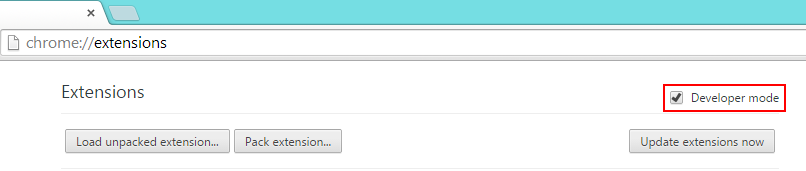
\includegraphics[width=1\textwidth]{figures/devmode.png}
	\caption{Enabling Chrome developer mode\label{fig:devmode}}
	\end{figure}

	\item Press the ``Load unpacked extension...'' button and select the folder containing your \texttt{manifest.json} file, as shown in \emph{Figure \ref{fig:loadext}}. Press ``OK'' to load your extension.\\

	\begin{figure}[htb]
	\centering
	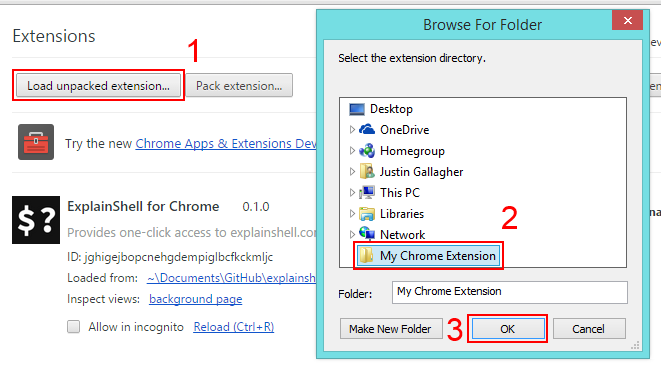
\includegraphics[height=0.5\textwidth]{figures/loadext.png}
	\caption{Adding your extension to Chrome\label{fig:loadext}}
	\end{figure}

	\item When your extension is properly loaded, you should see an entry for ``My Chrome Extension'' in the extensions list, as shown in \emph{Figure \ref{fig:loadedext}}.\\

	\begin{figure}[htb]
	\centering
	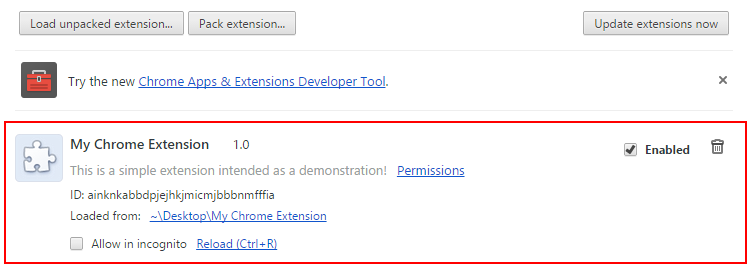
\includegraphics[width=1\textwidth]{figures/loadedext.png}
	\caption{A successfully loaded extension\label{fig:loadedext}}
	\end{figure}
\end{enumerate}

Now your extension has been loaded into the browser, and you should immediately see the extension you have written take effect.

Proceed to the next step to learn how to upload your extension to the Chrome Web Store for others to download.

\newpage

\section{Uploading the Extension to the Chrome Web Store}

This step shows you how to upload your app to the Chrome Web Store for others to download and use.

\begin{enumerate}
	\item Zip your extension directory. To do this in Windows, open Windows Explorer, right click on the directory, and choose ``Send to'', then click ``Compressed (zipped) folder'', as shown in \emph{Figure \ref{fig:zipext}}.\\

	\begin{figure}[htb]
	\centering
	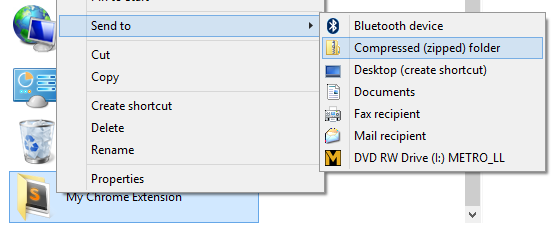
\includegraphics[width=0.7\textwidth]{figures/zipext.png}
	\caption{Zipping a directory in Windows Explorer\label{fig:zipext}}
	\end{figure}

	\item Navigate to the Chrome Web Store Developer Dashboard at \\\texttt{https://chrome.google.com/webstore/developer/dashboard}, and sign in to your Google Account.

	\item If this is your first time publishing an application through Google, you will need to pay Google's \$5 registration fee. A yellow banner will be displayed on the dashboard if you need to pay this fee, as in \emph{Figure \ref{fig:regfee}} - press the ``Pay this fee now'' button and follow Google's instructions to enable your developer account.\\

	\begin{figure}[htb]
	\centering
	
\includegraphics[width=1\textwidth]{figures/regfee.png}
	\caption{Google developer registration fee notice\label{fig:regfee}}
	\end{figure}

	\item Click the ``Add New Item'' button on the dashboard. Here, you will be prompted to upload your extension's \texttt{.zip} file, created in substep 1. Click ``Choose file'', and select the \texttt{.zip} file, as shown in \emph{Figure \ref{fig:uploadext}}. Press the ``Upload'' button to complete the transaction.\\

	\begin{figure}[htb]
	\centering
	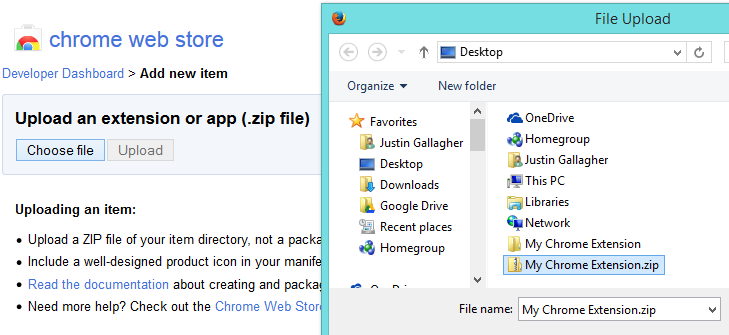
\includegraphics[width=0.7\textwidth]{figures/uploadext.png}
	\caption{Uploading your extension to Google\label{fig:uploadext}}
	\end{figure}

	\item You will now be redirected to a page where you can configure the store appearance of your extension. There are many options available on this page, but most are optional. Make sure you set the ``Category'' and ``Language'' fields of the form to appropriate values. Click ``Publish changes'' to publish your app to the Chrome store. It may take up to an hour for your extension to appear to others. When you are done, your extension will have a page in the Web Store as in \emph{Figure \ref{fig:publishedext}}.\\

	\begin{figure}[htb]
	\centering
	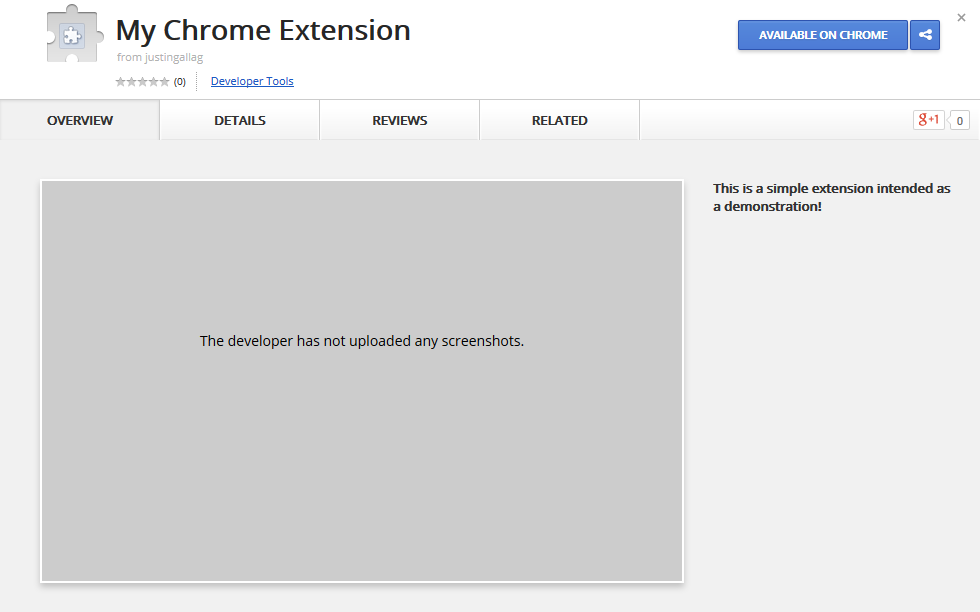
\includegraphics[width=0.7\textwidth]{figures/publishedext.png}
	\caption{Store page for a completed extension\label{fig:publishedext}}
	\end{figure}
\end{enumerate}

Your extension will now be available for public download, and can be found in the Chrome Web Store's search.

\end{document}
